\chapter{16s-rRNA Sequencing}
\pagenumbering{arabic} \setcounter{page}{9}

This section presents the science behind 16s-rRNA, how the sequencing is done in order to obtain reads. The section further elaborates on the OTUs and ASVs which are obtained after conducting a bioinformatics analysis. There has been a lot of dispute over the effectiveness of OTUs and ASVs in analyzing the microbial community. Hence, the present section also strives to explain the successes and limitations of both approaches

\subsection{16s ribosomal RNA}
The 16s-rRNA is the RNA part of the 30s small subunit of the ribosome (in prokaryotes).  Inside a prokaryotic cell, it is responsible for scaffolding the position of ribosomal proteins. It also binds to the shine-Dalgarno-Sequence to begin protein synthesis by utilising protein S1 and S21. The 16s-rRNA has seven highly conserved regions flanked by nine hypervariable regions, and therefore it is used in producing phylogenies. The slow rate of evolution 1500 bp long 16s-rRNA makes it a perfect nominee for taxonomic surveys. It is found to be competent in re-classifying prokaryotes into new species and genera. The V4 region is semi-conserved and is proficient in giving phylum-level classification. The V3 region identifies the genus' high accuracy, whereas the V6 is best at distinguishing species. The V1-V8 regions are most effective to include for a disease-specific assay. However, in the families Enterobacteriaceae, Clostridiaceae, and Peptostreptococcaceae, species can have high sequence similarity (99\%); therefore, the V4 sequences can fail to differentiate at lower taxonomic levels. For the taxonomic assignment, there exist highly curated and quality-controlled databases which microbiologists use to assign taxonomies.

\begin{itemize}
  \item \textit{SILVA Database}: It caters an extensive, quality-checked, \& updated datasets of ribosomal sequences for Bacteria, Archaea and Eukarya.
  \item \textit{Ribosomal Database Project (RDP)}: It stores QC passes, aligned and annotated seqs from bactria \& archeas and fungi (28S rRNA).
\end{itemize}

\subsection{16s Amplicon Sequencing}

\begin{enumerate}
  \item \textit{Sampling}: Like any other sequencing, a typical 16s Amplicon sequencing commences with the collection of samples. The samples are directly sourced from the site under study or extracted from the specimen (e.g. gut microbiome).
  \item \textit{Extraction of DNA}: The bulk-DNA is then extracted from the obtained samples using various commercialised preparation kits. The step is very crucial and is often prone to errors due to the presence of environmental DNAse. Therefore, care should be taken during DNA extraction.
  \item \textit{Library Preparation}: The extracted DNA is then sheared and is fragmented into pieces for PCR amplification. This enhances the copy number of the sequence of interest. This step is also prone to technical artefacts, which are somewhat unavoidable. 
  \item \textit{Adaptor Ligation and barcoding}: Adaptors are the known sequences attached along with the 3' and 5' end of the 16-rRNA hypervariable regions (specifically to the V4). The barcodes are added during a multi-plex run which helps in differentiating the samples.
  \item \textit{Sequencing}: Sequencing can be done by a traditional synthesis method, which produces fluorescent signals upon nucleotide addition. Semiconductor based methods like Ion-torrent were initially used however they were discarded as they were error-prone. Technologies like nano-pore, which make long reads, are becoming a standard as they cover the entire length of the 16s-rRNA gene. \textcolor{red}{Nowadays, Illumina sequencing-by-synthesis methodology is used, which, instead of 454 pyrosequencing, produces a lower per-base error and is not susceptive to indels-base errors \cite{ref14}.}
  \item \textit{Data Analysis}: The last step involves the data analysis using complex bioinformatics toolkits.This includes the generation of OTUs/ASVs, which can be further used to produce phylogenetic trees and draw conclusions.
\end{enumerate}

\begin{figure}[!hb]
  \centering
  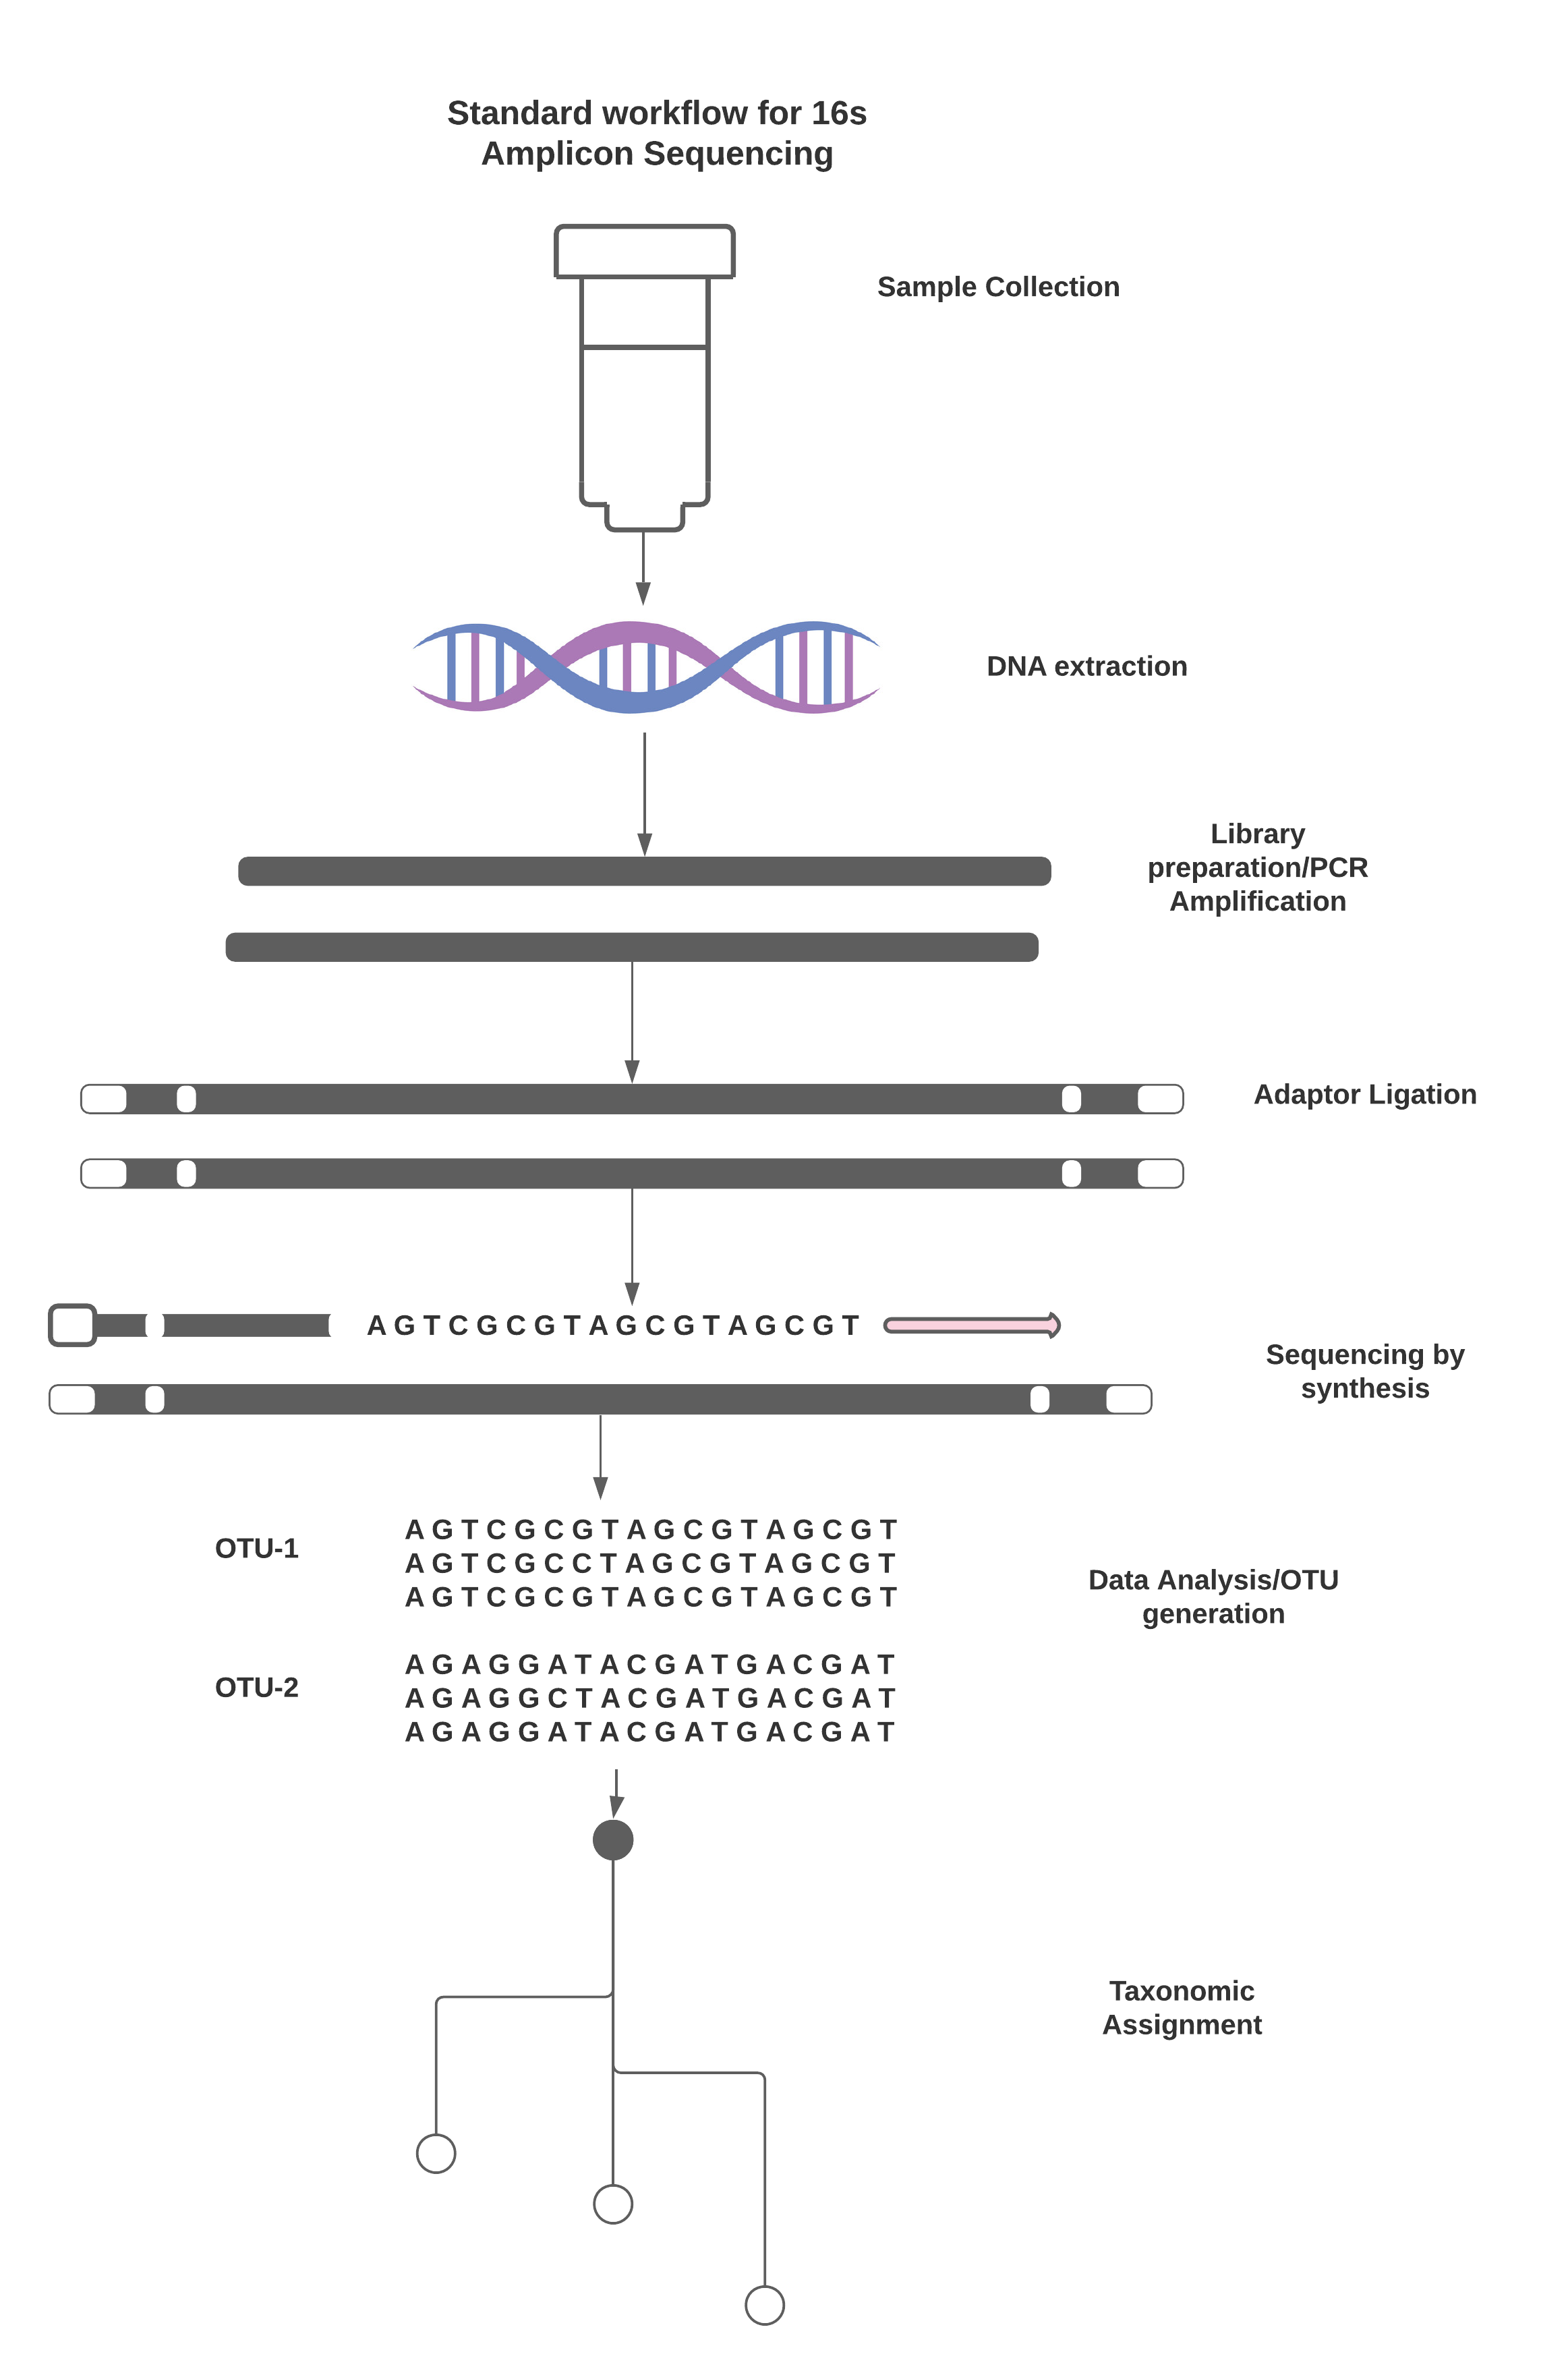
\includegraphics[width=10cm, height=15cm]{../figures/Figure3.png}
  \caption{Standard Workflow for 16s Amplicon Sequencing}
  \label{fig:figure3}
\end{figure}

\subsection{Operational Taxonomic Units}
OTUs are the clusters of sequenced reads that vary by a similarity cut-off. Arguably, the similarity threshold has been set to a constant of 97\% due to many use-cases from 1994. The OTUs thus made are the representatives of a group of sequence reads which are 3\% dissimilar. To be exact, OTUs are pragmatic proxies of the actual sequences read from the data. OTU clusters can either be made using a Hierarchical clustering algorithm such as UCLUST or CD-HIT, or they can be produced using Bayesian clustering approaches such as CROP. However, recent findings have shown that the threshold of 97\% is inefficient to draw ecologically valid conclusions from the data. There has been a dispute about whether the threshold should be tuned depending upon the quality of reads or samples. Even after being a highly questioned concept, the reference-based OTUs are \textcolor{green}{quite} accurate compared to de-novo OTUs. \textcolor{red}{OTU clustering can be done with or without using a database. Close reference clustering involves comparing sequences against a curated database, which are then clustered into OTUs \cite{ref15}. However, it suffers if the reference sequence is not present in the dataset. Strengths include the ability to compare OTU assignments across studies. De novo clustering methods calculates the distance between sequences which is then used to cluster sequences into OTUs \cite{ref15}. However, the computational cost scales quadratically with the number of unique sequences. Open-reference clustering also involves performing closed-reference clustering followed by de novo clustering on those sequences that are not sufficiently similar to the reference \cite{ref15}.}

\subsection{Amplicon Sequence Variants}
They are also called the Exact Sequence Variants (ESVs) or Zero-Radius OTUs (ZOTUs). They are 100\% non-identical rather than similar and provide a high-resolution picture as opposed to the OTUs as they are resolved down to the difference of one nucleotide \cite{ref16}. Using ASVs, one can detect microbes that may have diverged a million years ago. ASVs from different studies can be mixed if the sequence reads are obtained from a similar genetic locus or if the overlapping regions are trimmed before the merging. Even though ASVs seem to be a sounder option than the OTUs, they have some limitations \cite{ref16}. Firstly, the 16-rRNA gene has more than one copy inside a bacteria, which could vary by 4-base pairs; this will make 4 individual variants into the downstream analysis. Moreover, the complexity of the alpha and beta diversity increase which also further complicates the analysis \cite{ref16}.